\chapter{Testing}


\section{Introduction}
In our scenario test strategy is used to test the functionality of our system.  
In our system testing is going to be done at individual module level. Each module will be undergone to Unit Testing and expected result is supposed to be same as actual result.\\

% This section type your project contents 

\section{Validation Testing}
The process of evaluating software during the development process or at the end of the development process to determine whether it satisfies specified business requirements.\\
Validation Testing ensures that the product actually meets the client's needs. It can also be defined as to demonstrate that the product full fills its intended use when deployed on appropriate environment.\\

\pagebreak

\textbf{Test Cases Perform}
\begin{center}
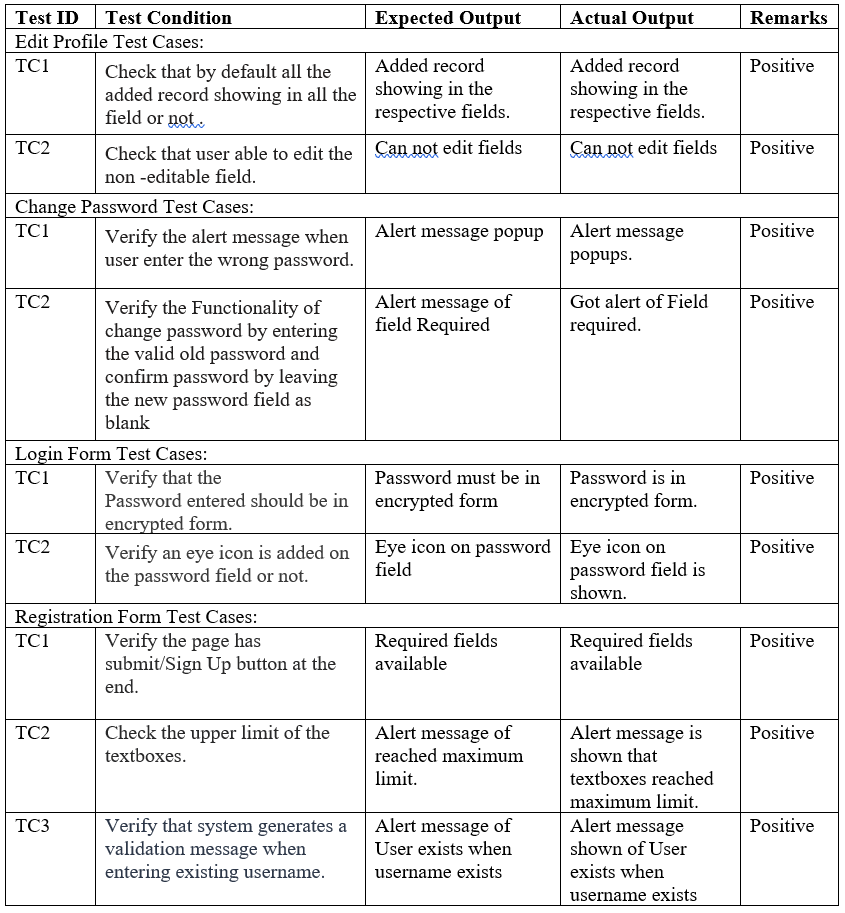
\includegraphics[height=16cm,width=14cm]{ch7/tc.png}
\end{center}



 